\documentclass{report}
\usepackage[T1]{fontenc}
\usepackage[utf8]{inputenc}
\usepackage{lmodern}
%\usepackage{hyperref}
\usepackage[portuges,brazilian]{babel}
\usepackage{graphicx}
\usepackage{textcomp}
\usepackage{fullpage}
\usepackage{wrapfig}
\usepackage{float}
\usepackage{listings}
\usepackage{amsmath}
\usepackage{amssymb}
\begin{document}

\newcommand{\HRule}{\rule{\linewidth}{0.5mm}}
\newcommand{\tsize}[1]{(\frac{W}{L})_{#1}}
 

%%%%%%%%%%%%%%%%%%%%%%%%%% START TITLE PAGE %%%%%%%%%%%%%%%%%%%%%%%%5
\begin{titlepage}

\begin{center}


{\LARGE UNIVERSIDADE DE SÃO PAULO\\}
{\LARGE DEPARTAMENTO DE ENGENHARIA ELÉTRICA \\}
{\LARGE ESCOLA DE ENGENHARIA DE SÃO CARLOS\\[4cm]}

\textbf{\large SEL5755 - Sistemas Fuzzy}\\[1cm]
\textbf{\large Prof Dr. Ivan Nunes da Silva}\\[2cm]


% Title
\HRule \\[0.6cm]
{ \huge EPC 2\bfseries }\\[0.6cm]

\HRule \\[2cm]

% Author

\begin{center} \large
\emph{Alunos:}\\
\end{center}

\begin{minipage}{0.4\textwidth}
\begin{flushleft} \large
Isabela R. do Prado \textsc{Rossales}\\
6445435
\end{flushleft}
\end{minipage}
\begin{minipage}{0.4\textwidth}
\begin{flushright} \large
Jonas Rossi \textsc{Dourado}\\
6445442
\end{flushright}
\end{minipage}

\vfill

% Bottom of the page
{\large São Carlos,\\ \today}

\end{center}

\end{titlepage}
%\listoffigures
%\begingroup
%\let\clearpage\relax
%\listoftables
%\endgroup
%%%%%%%%%%%%%%%%%%%%%%%%%% STOP TITLE PAGE %%%%%%%%%%%%%%%%%%%%%%%%5


\newpage

\begin{enumerate}

\item[1] Considere o conjunto \emph{fuzzy} A definido no universo de discurso $X = \{ x \in  \mathbb{R} \vert 0 \le x \le 10\}$,
o qual é representado pela seguinte função de pertinência:


\begin{equation*}
\mu_A (x) = 
\begin{cases} 
0,5x-1,5, & \text{se $3 \leq x \leq 5$}
\\
-0,5x+3,5, & \text{se $5 < x \leq 7$}
\\
0, &\text{caso contrário}
\end{cases}
\end{equation*}

\begin{enumerate}
    \item[a)] Esboce o gráfico da função de pertinência representada acima, indicando também qual é o seu tipo.

        \begin{figure}[hptb]
        \centering
        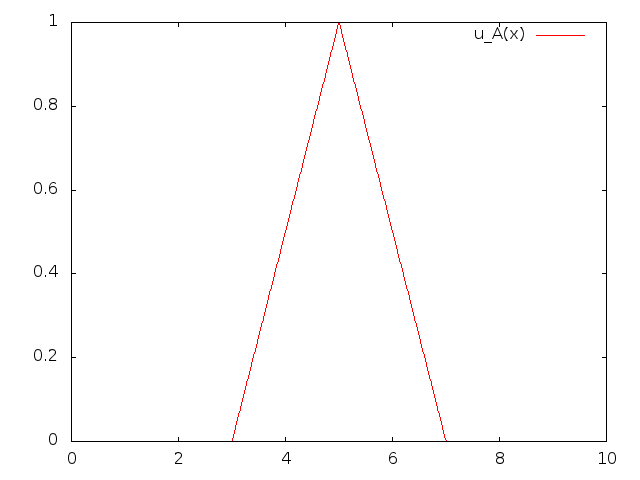
\includegraphics[scale=0.3]{ex1a.png}
        \caption{Função de pertinência.}
        \label{fig:1a}
        \end{figure}
    
    De acordo com o gráfico da função de pertinência (Figura \ref{fig:1a}), temos que seu tipo é triangular.
        

    \item[b)] Sabendo-se que a função acima está representando o conjunto referente à temperatura ``média'' de um determinado
    processo industrial, explique então qual o significado que está embutido em tal representação.

    De acordo com a representação, a temperatura média está em torno de 5 (unidade não especificada), mas com certeza não
    é menor que 3 ou maior que 7. 

    \item[c)] Explique se o conjunto \emph{fuzzy} acima é considerado um conjunto normalizado.

    O conjunto é normalizado porque pelo menos um de seus elementos possui grau de pertinência igual a 1 (elemento 5).


    \item[d)] Obtenha o conjunto suporte associado ao conjunto \emph{fuzzy} acima.

    $SUPP(A) = \{ x \in  \mathbb{R} \vert \mu_A(x) > 0\} = \{ x \in \mathbb{R} \vert x \in ]3;7[ \}$

\end{enumerate}

\item[2] Calcule a cardinalidade dos conjuntos \emph{fuzzy} discretos dados a seguir:
\begin{enumerate}
    \item[a)] $A = 0,3/x_1 + 0,5/x_2 + 0,9/x_3 + 0,4/x_4 + 0,1/x_5$

    $CARD(A) = 0,3+0,5+0,9+0,4+0,1 = 2,2 $

    \item[b)] $A = 0,0/x_1 + 0,4/x_2 + 1,0/x_3 + 1,0/x_4 + 0,4/x_5 + 0,0/x_6$

    $CARD(A) = 0,4 1,0+ 1,0 + 0,4 = 2,8$


    \item[c)] $\mu_c(x)=\frac{x}{x+1}, \text{com } x \in \{0,1,2,...,10 \}$

    $ CARD(A) = \sum\limits_{x=0}^{10}\mu_C(x) = 7,98$ 

\end{enumerate}


\item[3] Uma equipe de engenheiros e cientistas obteve a partir de experimentação diversos valores de
$\alpha$-cortes referentes a um conjunto \emph{fuzzy} V que está sendo mapeado, o qual está representando o
ajuste de vazão v de uma coluna de destilação de petróleo. Os valores referentes aos $\alpha$-cortes são
dados a seguir:\\
$V_{0.00} = \{v \in \Re / 2,0 \leq v \leq 8,0\}$\\
$V_{0.25} = \{v \in \Re / 2,5 \leq v \leq 7,5\}$\\
$V_{0.50} = \{v \in \Re / 3,0 \leq v \leq 7,0\}$\\
$V_{0.75} = \{v \in \Re / 3,5 \leq v \leq 6,5\}$\\
$V_{1.00} = \{v \in \Re / 4,0 \leq v \leq 6,0\}$\\
A partir das informações acima reconstrua um gráfico representativo deste conjunto, obtendo
ainda a sua expressão analítica.

\begin{figure}[hptb]
\centering
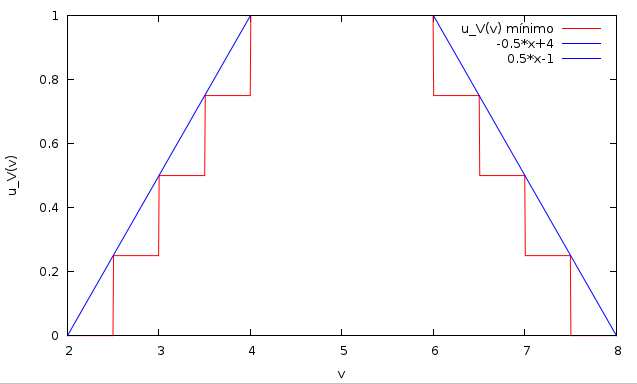
\includegraphics[scale=0.7]{ex3.png}
\caption{Gráfico representativo do conjunto.}
\label{fig:ex3}
\end{figure}

Conforme mostrado na Figura \ref{fig:ex3}, a expressão analítica da função de pertinência foi obtida através da
criação de uma função linear tal que $\mu_V(v)$ pertencesse aos valores máximos e mínimos determinados pelos 
$\alpha$-cortes. Temos que:

\begin{equation*}
\mu_V (v) = 
\begin{cases} 
0,5x-1, & \text{se $2 \leq v < 4$}
\\
1, & \text{se $4\le v \le 6$}
\\
-0,5x+4, & \text{se $6 < v \leq 8$}
\\
0, &\text{caso contrário}
\end{cases}
\end{equation*}


\item[4] Um determinado conjunto \emph{fuzzy} deverá ser mapeado utilizando função de pertinência
triangular ou trapezoidal. Discorra sobre que subsídios você usaria para escolher uma dessas
funções para representar este conjunto. Explicite os seus argumentos através de um exemplo.

Para escolher mapear um conjunto \emph{fuzzy} entre uma função de pertinência triangular ou uma trapezoidal
é necessário ter um conhecimento prévio por parte do projetista (que pode ser obtido a partir de experiência própria 
ou pesquisa). 

A partir do conhecimento prévio é possível decidir 
qual função se adéqua mais ao conjunto \emph{fuzzy} em questão. 
Se o conjunto a ser mapeado apresenta uma faixa de valores com grau de pertinência iguais, a função trapezoidal
é a mais indicada. Caso haja apenas um elemento com o valor do maior grau de pertinência, pode-se utilizar a função
triangular.

Por exemplo, temos a situação em que a velocidade do motor de uma centrífuga é representada
em um conjunto \emph{fuzzy} ``adequado à aplicação'' (universo de discurso de 0 rpm até 10000 rpm). 
O conjunto \emph{fuzzy} ``adequado à aplicação'' é razoável 
de ser mapeado
para uma função de pertinência trapezoidal pois em uma centrífuga há faixas de velocidade adequadas à opção escolhida pelo usuário.
Por outro lado, ao se dizer que a temperatura média em uma determinada cidade está em torno de $25^o$ C, 
a função mais indicada que mapeia o conjunto correspondente é a triangular.



\item[5] Explique se a afirmação seguinte é verdadeira ou falsa: “Se um conjunto \emph{fuzzy} contínuo em
seu universo de discurso tiver algum de seus $\alpha$-cortes também contínuo, então o referido
conjunto é considerado convexo”.

A afirmação apresentada no exercício é falsa pois pode haver $\alpha$-cortes que são contínuos e ainda assim 
existir $\alpha$-cortes deslocados por um $\theta$ qualquer ($A_{\alpha+\theta}$) que não são contínuos (caracterizando
assim um conjunto \emph{fuzzy} não convexo). Para tornar a afirmação verdadeira, seria necessário que \emph{todos} os seus $\alpha$-cortes 
fossem contínuos.


\end{enumerate}


\end{document}
